\documentclass[xcolor={dvipsnames},handout]{beamer}

\usepackage{assets/pres-template_MOW}
\usepackage{pdfpages}

%--------------------------------------------------------------------------
% Specific to this document ---------------------------------------
\usepackage{amsmath}
\usepackage{amssymb}

%--------------------------------------------------------------------------
% \setbeamercovered{transparent}

%%%%%%%%%%%%%%%%%%%%%%%%%%%%%%%%%%%
\setlength{\tabcolsep}{1.3pt}
\title{PLSC 48110/28110}
\subtitle{Lecture 6: Power calculations and randomization procedures}
\date{}
\author{Molly Offer-Westort}
\institute{Department of Political Science, \\University of Chicago}


\usepackage{assets/Sweave}
\renewcommand{\Sweavesize}{\scriptsize}
\renewcommand{\Routsize}{\scriptsize}
\hypersetup{pdftitle={PLSC 48110/28110 - Lecture 6: Power calculations and randomization procedures},pdfauthor={Molly Offer-Westort},pdfpagemode=UseNone}
\begin{document}

%-------------------------------------------------------------------------------%
\frame{\titlepage
\thispagestyle{empty}
}
%-------------------------------------------------------------------------------%
\begin{frame}{One-pager overview}

\begin{itemize}
\item See the syllabus for the submission deadline.
\item Meet with me to discuss; schedule a meeting at \url{https://calendly.com/mollyow/office-hours} 
\item One-pager should cover general research question, how you would think about answering it, and some general design considerations.  You are not directly graded on the one-pager, but it allows us to give you feedback to make your final project better. 
\item See Lecture 5 for design documents and pre-registrations.
\end{itemize}

\end{frame}


%%%%%NOTE%%%%%
\note{
\scriptsize \singlespacing

\begin{itemize}
\item xxxx
\end{itemize}

}

%-------------------------------------------------------------------------------%
\begin{frame}{Considerations when running an experiment}

\begin{itemize}
\item What hypotheses are you testing?  And what estimation techniques used to test them?
\item What proportion of subjects in treatment vs. control?  Or, with multiple conditions, what proportion in each? 
\item Oversampling some sub-populations? 
\item (Replicable) methods for randomization  (is your study online? in person? do you have the full sample frame ex ante?) 
\item Also: ethical considerations, cost, implementation barriers
\end{itemize}

\end{frame}


%%%%%NOTE%%%%%
\note{
\scriptsize \singlespacing

\begin{itemize}
\item xxxx
\end{itemize}

}

%-------------------------------------------------------------------------------%
\begin{frame}{Sample frame}

\begin{itemize}
\item Who is included in your study? How are they selected? 
\item Random selection?  Clustered selection ? (e.g., schools, neighborhoods)  Somehow representative of a population?  Convenience sample?  Eligibility criteria? 
\item Important for both internal and external validity. 
\item Approaches to creating a sample frame: 
\begin{itemize}
\item Administrative data (census, school registers, health data)
\item Do your own census/mapping exercise 
\item "Random walk"
\item Ongoing enrollment: online population, people at a health clinic;  generally have eligibility criteria
\end{itemize}
\end{itemize}

\end{frame}


%%%%%NOTE%%%%%
\note{
\scriptsize \singlespacing

\begin{itemize}
\item xxxx
\end{itemize}

}

%-------------------------------------------------------------------------------%

\begin{frame}{Randomization procedures}

\begin{itemize}
\item Simple random assignment
\item Complete random assignment 
\item Stratified random assignment 
\item Paired random assignment 
\item Clustered random assignment 
\end{itemize}

\end{frame}


%%%%%NOTE%%%%%
\note{
\scriptsize \singlespacing

\begin{itemize}
\item xxxx
\end{itemize}

}

%-------------------------------------------------------------------------------%
\begin{frame}{Randomization procedures: mechanisms}

\begin{itemize}
\item Is it replicable?  Is it public?  What could go wrong? 
\item Lottery 
\item Random walk 
\item Computer program
\end{itemize}

\end{frame}


%%%%%NOTE%%%%%
\note{
\scriptsize \singlespacing

\begin{itemize}
\item xxxx
\end{itemize}

}

%-------------------------------------------------------------------------------%
\begin{frame}{Simple random assignment}

\begin{itemize}
\item Treatment assignment probabilities are the same across units 
\item Treatment is assigned to each unit independently 
\item Not optimal for estimation $\rightarrow$ can have chance imbalance in treatment and control. 
\item But sometimes required in practice, e.g., when you don't have your entire sample frame prior to starting the experiment
\end{itemize}

\end{frame}


%%%%%NOTE%%%%%
\note{
\scriptsize \singlespacing

\begin{itemize}
\item xxxx
\end{itemize}

}

%-------------------------------------------------------------------------------%
\begin{frame}{Complete random assignment}

\begin{itemize}
\item Fix the number/proportion of units in treatment and control, then randomize over sample frame. 
\item We can still get chance imbalance on measured and unmeasured variables. 
\end{itemize}

\end{frame}


%%%%%NOTE%%%%%
\note{
\scriptsize \singlespacing

\begin{itemize}
\item xxxx
\end{itemize}

}

%-------------------------------------------------------------------------------%
\begin{frame}{Stratified random assignment}

\begin{itemize}
\item Divide your sample frame into subgroups.  Apply complete random assignment \textit{within} subgroups. 
\item Benefits: removes chance of imbalance on \textit{measured} variables.  Especially useful if we want to look at treatment effects within subgroups. 
\item Sometimes different strata have different assignment probabilities. 
\end{itemize}

\end{frame}


%%%%%NOTE%%%%%
\note{
\scriptsize \singlespacing

\begin{itemize}
\item xxxx
\end{itemize}

}

%-------------------------------------------------------------------------------%
\begin{frame}{Stratified random assignment}

\begin{itemize}
\item How do you decide what variables to stratify on, and where to bin continuous variables?
\item Variable should correlate with outcome variable. 
\item For binning, can use statistical methods (e.g., decision trees). 
\end{itemize}

\end{frame}


%%%%%NOTE%%%%%
\note{
\scriptsize \singlespacing

\begin{itemize}
\item xxxx
\end{itemize}

}

%-------------------------------------------------------------------------------%
\begin{frame}{Clustered random assignment}

\begin{itemize}
\item Divide your sample into subgroups. 
\item Assign treatment uniformly within subgroups.  (Or at fixed levels of treatment intensity.) 
\item Bias-variance trade-off. 
\item Useful when there is spillover, and/or you're interested in what a program would look like if implemented uniformly at scale. 
\item Setting different levels of treatment intensity can facilitate estimating spillovers as well as direct effects. \citep{baird2018optimal}
\end{itemize}

\end{frame}


%%%%%NOTE%%%%%
\note{
\scriptsize \singlespacing

\begin{itemize}
\item xxxx
\end{itemize}

}

%-------------------------------------------------------------------------------%
\begin{frame}{What about re-randomization?}

\begin{itemize}
\item What are criteria?
\end{itemize}

\end{frame}


%%%%%NOTE%%%%%
\note{
\scriptsize \singlespacing

\begin{itemize}
\item xxxx
\end{itemize}

}

%-------------------------------------------------------------------------------%
\begin{frame}{Power}

\begin{itemize}
\item How large does my experiment need to be for my proposed statistical procedure to be informative?  (under certain conditions) 
\item The test can be about distinguishing treatment effects from zero, but it doesn't \textit{have} to be. 
\item Hypothesis: alternative vs. null. 
\end{itemize}

\end{frame}


%%%%%NOTE%%%%%
\note{
\scriptsize \singlespacing

\begin{itemize}
\item xxxx
\end{itemize}

}

%-------------------------------------------------------------------------------%
\begin{frame}{Power}

\begin{itemize}
\item Type I error: falsely reject the null. Probability in terms of $\alpha$.
\item Type II error: fail to detect an effect when it exists. Probability in terms of $\beta$. 
\item Power: probability of rejecting a "false null hypothesis."  I.e., given that there \textit{is} an effect, do you correctly reject the null? Probability in terms of $1 - \beta$.  Often, we target power of $1-\beta$. 
\item Minimum detectable effect: the smallest effect that would produce our target power, given a specific statistical test and a given $\alpha$.  Selection often informed by substantive knowledge or policy relevance. 
\end{itemize}

\end{frame}


%%%%%NOTE%%%%%
\note{
\scriptsize \singlespacing

\begin{itemize}
\item xxxx
\end{itemize}

}

%-------------------------------------------------------------------------------%
\begin{frame}{Power}

\begin{figure}
\centering
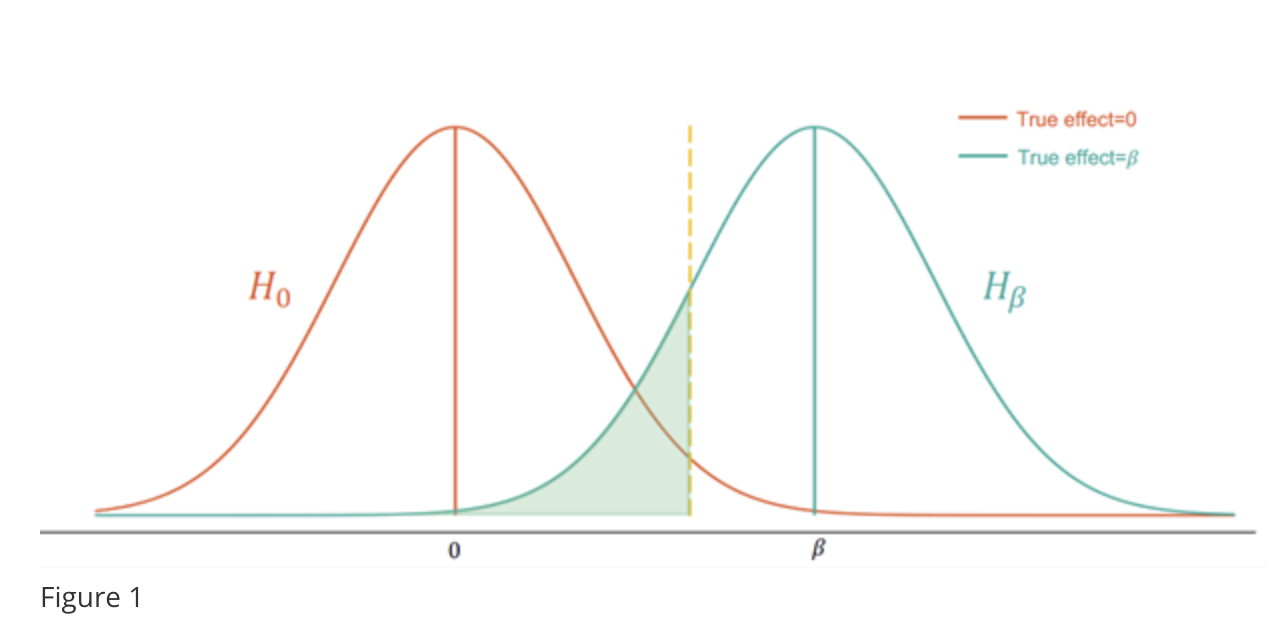
\includegraphics[]{assets/power_plot.png}
\end{figure}

\end{frame}


%%%%%NOTE%%%%%
\note{
\scriptsize \singlespacing

\begin{itemize}
\item xxxx
\end{itemize}

}

%-------------------------------------------------------------------------------%
\begin{frame}{Power}

Note: power is with respect to:
\begin{itemize}
\item Statistical elements: a given statistical test, a given $\alpha$, a given minimum detectable effect size, a given sample size.  We also need to specify the statistical distribution of our response variable. 
\begin{itemize}
\item Distributions: normal, binomial.  Intra-cluster correlation? 
\end{itemize}
\item Design elements: sample size, treatment allocation. 
\end{itemize}

\end{frame}


%%%%%NOTE%%%%%
\note{
\scriptsize \singlespacing

\begin{itemize}
\item xxxx
\end{itemize}

}

%-------------------------------------------------------------------------------%
\begin{frame}[fragile]{Example}

\scriptsize
\begin{Schunk}
\begin{Sinput}
> library(ggplot2) 
> library(estimatr) # for lin estimator
> set.seed(60637) # setting a seed is important
> complete_assign <- function(n){
+   quotient <- n %/% 2
+   remainder <- n %% 2
+   
+   c(sample(rep(c(0,1), quotient)), 
+     sample(0:1, size = remainder))
+ }
\end{Sinput}
\end{Schunk}


\end{frame}


%%%%%NOTE%%%%%
\note{
\scriptsize \singlespacing

\begin{itemize}
\item xxxx
\end{itemize}

}

%-------------------------------------------------------------------------------%
\begin{frame}{Example}

You can use the \texttt{randomizr} package in \texttt{R}. It has functions like \texttt{complete\_ra()} to implement complete random assignment. 

\end{frame}


%%%%%NOTE%%%%%
\note{
\scriptsize \singlespacing

\begin{itemize}
\item xxxx
\end{itemize}

}

%-------------------------------------------------------------------------------%
\begin{frame}{Example}

Suppose:
\begin{itemize}
\item We have $n = 100$ observations in our sample. 
\item We assign treatment $W$ to half of the sample using complete random assignment. 
\item There is an $X$ variable distributed $\mathcal{N}(0,1)$
\item The treatment effect $\tau$ is equal to 2. 
\item Individual response follows:
\[
Y = 3X + \tau \times W + \epsilon
\]
Where $\epsilon$ is random noise distributed $\mathcal{N}(0,1)$.
\end{itemize}

\end{frame}


%%%%%NOTE%%%%%
\note{
\scriptsize \singlespacing

\begin{itemize}
\item xxxx
\end{itemize}

}

%-------------------------------------------------------------------------------%

\begin{frame}[fragile]{Example}

\scriptsize
\begin{Schunk}
\begin{Sinput}
> n <- 1e2
> W <- complete_assign(n)
> X <- rnorm(mean = 0, sd = 1, n = n)
> tau <- 2
> Y <- 3*X + tau*W + rnorm(mean = 0, sd = 1, n = n)
\end{Sinput}
\end{Schunk}


\end{frame}


%%%%%NOTE%%%%%
\note{
\scriptsize \singlespacing

\begin{itemize}
\item xxxx
\end{itemize}

}

%-------------------------------------------------------------------------------%
\begin{frame}[fragile]{Example}

We consider both $X$, and a dichotomized variable $\tilde X$, which is 1 when $X>0$ and 0 if $X<0$. 

\scriptsize
\begin{Schunk}
\begin{Sinput}
> Xtilde <- 1*(X>0)
\end{Sinput}
\end{Schunk}



\begin{Schunk}
\begin{Sinput}
> dat <- data.frame(Y, W, X, Xtilde)
> head(dat)
\end{Sinput}
\begin{Soutput}
           Y W           X Xtilde
1 -0.3918746 1 -0.29282895      0
2  0.1056477 1 -0.49140540      0
3  1.5193091 0  0.15595692      1
4  0.5207658 0  0.08337197      1
5  5.8685348 0  2.31585521      1
6  2.0938111 1  0.04878741      1
\end{Soutput}
\end{Schunk}

\end{frame}


%%%%%NOTE%%%%%
\note{
\scriptsize \singlespacing

\begin{itemize}
\item xxxx
\end{itemize}

}

%-------------------------------------------------------------------------------%
\begin{frame}[fragile]{Example}

We can estimate our treatment effect as a difference in means. 

\scriptsize
\begin{Schunk}
\begin{Sinput}
> difference_in_means(Y ~W, data = dat) # from estimatr
\end{Sinput}
\begin{Soutput}
Design:  Standard 
  Estimate Std. Error  t value    Pr(>|t|)
W 1.709098  0.6167788 2.771006 0.006705978

  CI Lower CI Upper       DF
W 0.4848694 2.933327 96.41715
\end{Soutput}
\end{Schunk}


\begin{Schunk}
\begin{Sinput}
> mean(Y[W == 1] - mean(Y[W == 0])) # equivalent
\end{Sinput}
\begin{Soutput}
[1] 1.709098
\end{Soutput}
\end{Schunk}


\end{frame}


%%%%%NOTE%%%%%
\note{
\scriptsize \singlespacing

\begin{itemize}
\item xxxx
\end{itemize}

}

%-------------------------------------------------------------------------------%
\begin{frame}{Example}

\begin{itemize}
\item How is precision affected if we had used a different design?  A different estimator? 
\item We will consider simple random assignment, complete random assignment, stratified random assignment, and paired random assignment. 
\end{itemize}

\end{frame}


%%%%%NOTE%%%%%
\note{
\scriptsize \singlespacing

\begin{itemize}
\item xxxx
\end{itemize}

}

%-------------------------------------------------------------------------------%
\begin{frame}[fragile]{Example}

\scriptsize
\begin{Schunk}
\begin{Sinput}
> niter <- 1e4
> estimates <- estimates_alt <- power <- power_alt <- matrix(NA, 
+   nrow = niter, 
+   ncol = 4)
> colnames(estimates) <- colnames(estimates_alt) <- colnames(power) <- 
+   colnames(power_alt) <- c('simple', 'complete', 'stratified', 'paired')
\end{Sinput}
\end{Schunk}


\end{frame}


%%%%%NOTE%%%%%
\note{
\scriptsize \singlespacing

\begin{itemize}
\item xxxx
\end{itemize}

}

%-------------------------------------------------------------------------------%
\begin{frame}[fragile]{Simulation: Simple random assignment}
\scriptsize
\begin{Schunk}
\begin{Sinput}
> for(i in 1:niter){
+   X <- rnorm(mean = 0, sd = 1, n = n)
+   Xtilde <- 1*(X>0)
+   
+   # Simple random assignment
+   W <- sample(0:1, size = n, replace = TRUE)
+   Y <- 3*X + tau*W + rnorm(mean = 0, sd = 1, n = n) 
+ 
+   est0 <- difference_in_means(Y~W, data = data.frame(Y, W))
+   est1 <- lm_lin(Y~W, covariates = formula('~ Xtilde'), 
+                  data = data.frame(Y, W, Xtilde))
+   estimates[i, 1] <- coef(est0)
+   power[i, 1] <- (est0$conf.low > 0 | est0$conf.high < 0)
+   estimates_alt[i, 1] <- coef(est1)[['W']]
+   power_alt[i, 1] <- (est1$conf.low['W'] > 0 | est1$conf.high['W'] < 0)
+
\end{Sinput}
\end{Schunk}
\end{frame}

\begin{frame}[fragile]{Simulation: Complete random assignment}
\scriptsize
\begin{Schunk}
\begin{Sinput}
+   # Complete random assignment
+   W <- complete_assign(n)
+   Y <- 3*X + tau*W + rnorm(mean = 0, sd = 1, n = n)
+   
+   est0 <- difference_in_means(Y~W, data = data.frame(Y, W))
+   est1 <- lm_lin(Y~W, covariates = formula('~ Xtilde'), 
+                  data = data.frame(Y, W, Xtilde))
+   estimates[i, 2] <- coef(est0)
+   power[i, 2] <- (est0$conf.low > 0 | est0$conf.high < 0)
+   estimates_alt[i, 2] <- coef(est1)[['W']]
+   power_alt[i, 2] <- (est1$conf.low['W'] > 0 | est1$conf.high['W'] < 0)
+
\end{Sinput}
\end{Schunk}
\end{frame}

\begin{frame}[fragile]{Simulation: Stratified random assignment}
\scriptsize
\begin{Schunk}
\begin{Sinput}
+   # Stratified random assignment
+   W <- rep(NA, n)
+   W[which(Xtilde == 0)] <-  complete_assign(sum((Xtilde == 0))) 
+   W[which(Xtilde == 1)] <-  complete_assign(sum((Xtilde == 1)))
+   Y <- 3*X + tau*W + rnorm(mean = 0, sd = 1, n = n)
+   
+   est0 <- difference_in_means(Y~W, data = data.frame(Y, W))
+   est1 <- lm_lin(Y~W, covariates = formula('~ Xtilde'), 
+                  data = data.frame(Y, W, Xtilde))
+   estimates[i, 3] <- coef(est0)
+   power[i, 3] <- (est0$conf.low > 0 | est0$conf.high < 0)
+   estimates_alt[i, 3] <- coef(est1)[['W']]
+   power_alt[i, 3] <- (est1$conf.low['W'] > 0 | est1$conf.high['W'] < 0)
+
\end{Sinput}
\end{Schunk}
\end{frame}

\begin{frame}[fragile]{Simulation: Paired random assignment}
\scriptsize
\begin{Schunk}
\begin{Sinput}
+   # Paired random assignment
+   W[order(X)] <- as.vector(replicate(n/2, sample(0:1)))
+   Y <- 3*X + tau*W + rnorm(mean = 0, sd = 1, n = n)
+   
+   est0 <- difference_in_means(Y~W, data = data.frame(Y, W))
+   est1 <- lm_lin(Y~W, covariates = formula('~ Xtilde'), 
+                  data = data.frame(Y, W, Xtilde))
+   estimates[i, 4] <- coef(est0)
+   power[i, 4] <- (est0$conf.low > 0 | est0$conf.high < 0)
+   estimates_alt[i, 4] <- coef(est1)[['W']]
+   power_alt[i, 4] <- (est1$conf.low['W'] > 0 | est1$conf.high['W'] < 0)
+ }
\end{Sinput}
\end{Schunk}
\end{frame}


%%%%%NOTE%%%%%
\note{
\scriptsize \singlespacing

\begin{itemize}
\item xxxx
\end{itemize}

}

%-------------------------------------------------------------------------------%
% The complete simulation loop appears across the preceding four frames.


%%%%%NOTE%%%%%
\note{
\scriptsize \singlespacing

\begin{itemize}
\item xxxx
\end{itemize}

}

%-------------------------------------------------------------------------------%

\begin{frame}[fragile]{Simulation results: variation}

\scriptsize
Variation of the estimate
\begin{Schunk}
\begin{Sinput}
> apply(estimates, 2, sd) # using difference in means estimate
\end{Sinput}
\begin{Soutput}
    simple   complete stratified     paired 
 0.6318423  0.6280029  0.4175988  0.2090756 
\end{Soutput}
\begin{Sinput}
> apply(estimates_alt, 2, sd) # using lin estimator
\end{Sinput}
\begin{Soutput}
    simple   complete stratified     paired 
 0.4195849  0.4140832  0.4145191  0.2188332 
\end{Soutput}
\end{Schunk}

\end{frame}

\begin{frame}[fragile]{Simulation results: power}
\scriptsize
\begin{Schunk}
\begin{Sinput}
> apply(power, 2, mean) # using difference in means estimate
\end{Sinput}
\begin{Soutput}
    simple   complete stratified     paired 
    0.8779     0.8839     0.9572     0.9994 
\end{Soutput}
\begin{Sinput}
> apply(power_alt, 2, mean) # using lin estimator
\end{Sinput}
\begin{Soutput}
    simple   complete stratified     paired 
    0.9966     0.9979     0.9973     1.0000 
\end{Soutput}
\end{Schunk}

\end{frame}


%%%%%NOTE%%%%%
\note{
\scriptsize \singlespacing

\begin{itemize}
\item xxxx
\end{itemize}

}

%-------------------------------------------------------------------------------%
\begin{frame}{How do you conduct power in practice?}

\begin{itemize}
\item Determine the appropriate minimum detectable effect size. 
\item Determine your estimating procedure. 
\item Posit a response distribution. 
\item Simulate over different sample sizes. 
\item OR, if simple, use an online power calculations calculator. 
\end{itemize}

\end{frame}


%%%%%NOTE%%%%%
\note{
\scriptsize \singlespacing

\begin{itemize}
\item xxxx
\end{itemize}

}

%-------------------------------------------------------------------------------%
%-------------------------------------------------------------------------------%


\backupbegin
%-------------------------------------------------------------------------------%

\begin{frame}[allowframebreaks]{References}
    \bibliographystyle{apalike}
    \bibliography{assets/bib}
\end{frame}
%-------------------------------------------------------------------------------%
\backupend
\end{document}
